\newcommand{\usecase}[7]{
\begin{center}
\begin{tabular}[h!]{| l | p{12cm} |}
	\hline
	\textbf{Name} & #1 \\ \hline
	\textbf{Actors} & #2 \\ \hline
	\textbf{Goal} & #3 \\ \hline
	\textbf{Preconditions} & #4 \\ \hline
	\textbf{Basic Flow} & #5 \\ \hline
	\textbf{Alternative Flow} & #6 \\ \hline
	\textbf{Postconditions} & #7 \\ \hline
\end{tabular}
\end{center}
}

\section{Use Case Diagram}

\begin{figure}[h!]
\begin{center}
	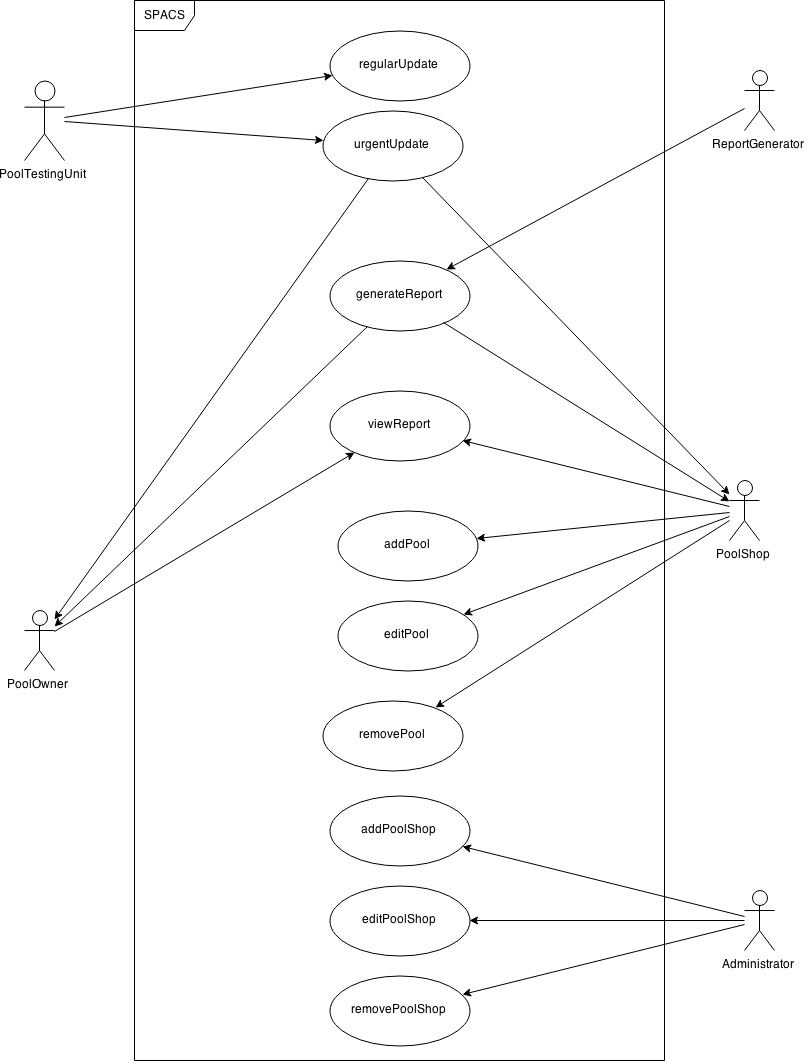
\includegraphics[width=13cm]{images/UseCaseDiagram}
	\caption{use case diagram outlining the main uses for the system}
\end{center}
\end{figure}


\usecase
{regular\_update}
{PoolTestingUnit}
{Store information received from the PoolTestingUnit in the system.}
{PoolTestingUnit is authenticated}
{
\begin{enumerate}
\item Use case starts when PTU sends data.
\item Data is checked for any errors.
\item Records from the data are stored for later analysis.
\item Use case ends.
\end{enumerate}
}
{
\begin{enumerate}
\item The data does not validate
\begin{enumerate}
\item The data is logged for analysis by support.
\end{enumerate}
\end{enumerate}
}
{\begin{enumerate}
\item Success: Data has been stored.
\item Failure: Data has been stored in a log for analysis by an Administrator.
\end{enumerate}
}

\usecase
{urgent\_update}
{PoolTestingUnit, PoolShop, PoolOwner}
{Store collected information received from the PoolTestingUnit in the system and alert the PoolOwner and PoolShop that there is a problem.}
{PoolTestingUnit is authenticated}
{
\begin{enumerate}
\item Use case starts when PoolTestingUnit sends data with alerts.
\item Data is checked for any errors.
\item Records from the data are stored for later analysis.
\item An email is sent to the PoolShopOwner and PoolOwner.
\item Use case ends.
\end{enumerate}
}
{
\begin{enumerate}
\item The data does not validate
\begin{enumerate}
\item Received data is logged for analysis
\item Email has been sent to PoolShopOwner and PoolOwner
\end{enumerate}
\end{enumerate}
}
{
\begin{enumerate}
\item Success: Data has been stored and an email has been sent to PoolShopOwner and PoolOwner.
\item Failure: Data has been stored in a log for analysis by an Administrator and an email has been sent to PoolShopOwner and PoolOwner.
\end{enumerate}
}

\usecase
{generate\_report}
{ReportGenerator, PoolOwner, PoolShopAdministrator}
{Provide latest data to the }
{First week of the PTU or a month since the last report for each pool}
{
\begin{enumerate}
\item Use case starts at the same time every day.
\item Gets a list of pools that need reports generated.
\item For report that needs generating:
\begin{enumerate}
\item Gets the information that should be on the report.
\item Generates the report as a pdf.
\item Emails the report off.
\item Saves a copy of the report for future reference.
\end{enumerate}
\end{enumerate}
}
{
\begin{enumerate}
\item Error generating report
\begin{enumerate}
\item Failure is logged for analysis by Administrator.
\end{enumerate}
\end{enumerate}
}
{
\begin{enumerate}
\item Success: Report generated and emailed to pool owner and pool shop
\item Failure: Any errors logged for admin to look over
\end{enumerate}
}

\usecase
{add\_pool\_shop}
{Administrator, PoolShop}
{To add a pool shop to the system.}
{Administrator is authenticated.}
{
\begin{enumerate}
\item Use case starts when an Administrator goes to the add pool shop page.
\item Administrator user enters information about the pool shop.
\item Information is validated to check for errors.
\item Information is stored and a new PoolShop is created.
\end{enumerate}
}
{
\begin{enumerate}
\item Invalid Information
\begin{enumerate}
\item Administrator user is informed
\item Administrator can modify information and try again.
\end{enumerate}
\end{enumerate}
}
{
\begin{enumerate}
\item Success: Information is stored and a new PoolShop is created.
\item Failure: No change to the system.
\end{enumerate}
}

\usecase
{edit\_pool\_shop}
{Administrator, PoolShop}
{To edit a pool shop in the system.}
{Administrator is authenticated.}
{
\begin{enumerate}
\item Use case starts when an Administrator goes to the edit pool shop page.
\item Administrator user changes information about the pool shop.
\item Information is validated to check for errors.
\item Information is stored and a PoolShop is updated.
\end{enumerate}
}
{
\begin{enumerate}
\item Invalid Information
\begin{enumerate}
\item Administrator user is informed
\item Administrator can modify information and try again.
\end{enumerate}
\end{enumerate}
}
{
\begin{enumerate}
\item Success: Information is stored and PoolShop is updated.
\item Failure: No change to the system.
\end{enumerate}
}

\usecase
{remove\_pool\_shop}
{Administrator, PoolShop}
{To remove a pool shop from the system.}
{Administrator is authenticated.}
{
\begin{enumerate}
\item Use case starts when an Administrator goes to the remove pool shop page.
\item Administrator confirms they want to remove PoolShop.
\end{enumerate}
}
{
\begin{enumerate}
\item Action Canceled
\begin{enumerate}
\item No change to the system.
\end{enumerate}
\end{enumerate}
}
{
\begin{enumerate}
\item Success: PoolShop is no longer usable.
\item Failure: No change to the system.
\end{enumerate}
}

\usecase
{add\_pool}
{PoolShop, PoolTestingUnit}
{To add a pool to the system.}
{PoolShop is authenticated.}
{
\begin{enumerate}
\item Use case starts when a PoolShop goes to the add pool page.
\item PoolShop user enters information about the pool.
\item Information is validated to check for errors.
\item Information is stored and a new PoolTestingUnit is created for the pool.
\end{enumerate}
}
{
\begin{enumerate}
\item Invalid Information
\begin{enumerate}
\item PoolShop user is informed
\item PoolShop can modify information and try again.
\end{enumerate}
\end{enumerate}
}
{
\begin{enumerate}
\item Success: Information is stored and a new PoolTestingUnit is created.
\item Failure: No change to the system.
\end{enumerate}
}

\usecase
{edit\_pool}
{PoolShop, PoolTestingUnit}
{To edit a pool in the system.}
{PoolShop is authenticated.}
{
\begin{enumerate}
\item Use case starts when a PoolShop goes to the edit pool page.
\item PoolShop user changes information about the pool shop.
\item Information is validated to check for errors.
\item Information is stored and a PoolTestingUnit is updated.
\end{enumerate}
}
{
\begin{enumerate}
\item Invalid Information
\begin{enumerate}
\item PoolShop user is informed
\item PoolShop can modify information and try again.
\end{enumerate}
\end{enumerate}
}
{
\begin{enumerate}
\item Success: Information is stored and PoolTestingUnit is updated.
\item Failure: No change to the system.
\end{enumerate}
}

\usecase
{remove\_pool}
{PoolShop, PoolTestingUnit}
{To remove a pool from the system.}
{PoolShop is authenticated.}
{
\begin{enumerate}
\item Use case starts when and PoolShop goes to the remove pool page.
\item PoolShop confirms they want to remove PoolTestingUnit.
\end{enumerate}
}
{
\begin{enumerate}
\item Action Canceled
\begin{enumerate}
\item No change to the system.
\end{enumerate}
\end{enumerate}
}
{
\begin{enumerate}
\item Success: PoolTestingUnit is no longer usable.
\item Failure: No change to the system.
\end{enumerate}
}

